\paragraph{样例图片}

\begin{center}
    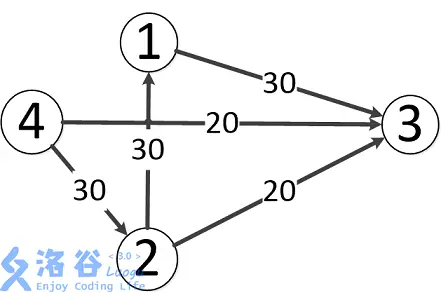
\includegraphics[width=0.4\textwidth]{img/luogu-P3376-1.png}
\end{center}

\paragraph{复杂度} \(O\left(|V|^2|E|\right)\)

\paragraph{无源汇上下界可行流} 给定无源汇流量网络 \(G\)~\\

询问是否存在一种标定每条边流量的方式, 使得每条边流量满足上下界同时每一个点流量平衡

不妨假设每条边已经流了 \(b(u,v)\) 的流量, 设其为初始流. 同时我们在新图中加入 \(u\) 连向 \(v\) 的流量为 $c(u,v) - b(u,v)$ 的边. 考虑在新图上进行调整

由于最大流需要满足初始流量平衡条件, 但是构造出来的初始流很有可能不满足初始流量平衡.

假设一个点初始流入流量减初始流出流量为 \(M\)

若 \(M=0\), 此时流量平衡, 不需要附加边

若 \(M>0\), 此时入流量过大, 需要新建附加源点 \(S'\), \(S'\) 向其连流量为 \(M\) 的附加边

若 \(M<0\), 此时出流量过大, 需要新建附加汇点 \(T'\), 其向 \(T'\) 连流量为 \(-M\) 的附加边

如果附加边满流, 说明这一个点的流量平衡条件可以满足, 否则这个点的流量平衡条件不满足

在建图完毕之后跑 \(S'\) 到 \(T'\) 的最大流, 若 \(S'\) 连出去的边全部满流, 则存在可行流, 否则不存在

\paragraph{有源汇上下界可行流} 给定有源汇流量网络 \(G\)~\\

询问是否存在一种标定每条边流量的方式, 使得每条边流量满足上下界同时除了源点和汇点每一个点流量平衡

假设源点为 \(S\), 汇点为 \(T\)

则我们可以加入一条 \(T\) 到 \(S\) 的上界为 \(\infty\), 下界为 \(0\) 的边转化为无源汇上下界可行流问题

若有解, 则 \(S\) 到 \(T\) 的可行流流量等于 \(T\) 到 \(S\) 的附加边的流量

\paragraph{有源汇上下界最大流} 给定有源汇流量网络 \(G\)~\\

询问是否存在一种标定每条边流量的方式, 使得每条边流量满足上下界同时除了源点和汇点每一个点流量平衡

如果存在, 询问满足标定的最大流量

我们找到网络上的任意一个可行流. 如果找不到解就可以直接结束

否则我们考虑删去所有附加边之后的残量网络并且在网络上进行调整

我们在残量网络上再跑一次 \(S\) 到 \(T\) 的最大流, 将可行流流量和最大流流量相加即为答案

\(S\) 到 \(T\) 的最大流直接在跑完有源汇上下界可行的残量网络上跑

千万不可以在原来的流量网络上跑

\paragraph{有源汇上下界最小流} 给定有源汇流量网络 \(G\)~\\

询问是否存在一种标定每条边流量的方式, 使得每条边流量满足上下界同时除了源点和汇点每一个点流量平衡

如果存在, 询问满足标定的最小流量

类似的, 我们考虑将残量网络中不需要的流退掉

我们找到网络上的任意一个可行流. 如果找不到解就可以直接结束

否则我们考虑删去所有附加边之后的残量网络

我们在残量网络上再跑一次 \(T\) 到 \(S\) 的最大流, 将可行流流量减去最大流流量即为答案